\documentclass[10pt,a4paper]{article}

% --- Packages ---
\usepackage[utf8]{inputenc}
\usepackage[T1]{fontenc}
\usepackage{lmodern}
\usepackage[margin=1.6cm,headheight=13pt]{geometry}
\usepackage{amsmath,amssymb}
\usepackage{graphicx}
\usepackage{booktabs}
\usepackage{tabularx}
\usepackage{microtype}
\usepackage{xcolor}
\usepackage{fancyhdr}
\usepackage{titlesec}
\usepackage{caption}
\usepackage{placeins}
\usepackage{cite}
\usepackage[colorlinks=true,linkcolor=blue!75!black,citecolor=blue!75!black,urlcolor=blue!75!black]{hyperref}

% --- Color Definitions ---
\definecolor{foamBlue}{RGB}{0,51,102}
\definecolor{slateGray}{RGB}{60,70,80}

% --- Header & Footer ---
\pagestyle{fancy}
\fancyhf{}
\fancyhead[L]{\footnotesize\color{slateGray}\textbf{CFD Final Project} --- Water-Cooled Duct Investigation}
\fancyhead[R]{\footnotesize\color{slateGray}OpenFOAM v2506}
\fancyfoot[L]{\footnotesize\color{slateGray}Parts I--V Summary Report}
\fancyfoot[R]{\footnotesize\color{slateGray}\thepage}
\renewcommand{\headrulewidth}{0.4pt}
\renewcommand{\footrulewidth}{0.4pt}

% --- Compact Section & Float Formatting ---
\titleformat{\section}{\color{foamBlue}\large\bfseries}{\thesection.}{0.5em}{}[\titlerule]
\titlespacing*{\section}{0pt}{1.1ex plus 0.4ex minus 0.2ex}{0.7ex plus 0.2ex}
\titleformat{\subsection}{\color{slateGray}\normalsize\bfseries}{\thesubsection}{0.4em}{}
\titlespacing*{\subsection}{0pt}{0.8ex plus 0.3ex minus 0.2ex}{0.4ex plus 0.1ex}

\captionsetup{font=small,labelfont=bf,skip=3pt}
\setlength{\textfloatsep}{8pt plus 2pt minus 2pt}
\setlength{\floatsep}{6pt plus 2pt minus 2pt}
\setlength{\intextsep}{7pt plus 2pt minus 2pt}
\setlength{\parindent}{0pt}
\setlength{\parskip}{3pt}

\begin{document}

% =============================================================================
% COMPACT HEADER
% =============================================================================
\begin{center}
    {\large\bfseries\color{foamBlue} CFD COURSE FINAL PROJECT}\\[0.2em]
    {\Large\bfseries Flow, Turbulence, and Heat Transfer from a Heated Block in a Water-Cooled Duct}\\[0.25em]
    {\small\color{slateGray} Parts I--V Required Results Report \quad|\quad \texttt{kOmegaSST} Low-$Re$ RANS / URANS / Multi-Region CHT}
\end{center}
\vspace{-0.3em}
\par\noindent\rule{\textwidth}{0.4pt}\par\vspace{0.2em}
\noindent{\footnotesize\begin{tabularx}{\textwidth}{@{}X X@{}}
    \textbf{Solvers:} \texttt{simpleFoam}, \texttt{pimpleFoam}, \texttt{chtMultiRegion(Simple)Foam} &
    \textbf{Water ($25\,^\circ\text{C}$):} $\rho = 1000\,\text{kg/m}^3$, $\mu = 8.90\times 10^{-4}\,\text{Pa}\cdot\text{s}$, $c_p = 4184\,\text{J/(kg}\cdot\text{K)}$, $\mathrm{Pr} = 6.135$ \\
    \textbf{Duct:} $0.20\times 0.20\times 1.50\,\text{m}$ ($D_h = 0.20\,\text{m}$, $L/D_h = 7.5$) &
    \textbf{Cube:} $H_c = 0.05\,\text{m}$ at $z\in[0.40,0.45]\,\text{m}$, $\dot{q} = 2.68\times 10^{10}\,\text{W/m}^3$ ($3.350\,\text{MW}$) \\
    \textbf{Turbulence:} Menter $k$-$\omega$ SST (Low-$Re$, $y^+_{\text{avg}} \le 1.0$) &
    \textbf{Flow:} $U_b = 1.00\,\text{m/s}$, $\dot{m} = 40.00\,\text{kg/s}$, $Re_{D_h} = 223{,}964$, $Re_{H_c} = 55{,}991$ \\
\end{tabularx}}\par\vspace{0.15em}
\noindent\rule{\textwidth}{0.4pt}

% =============================================================================
% SECTION 1: PART I
% =============================================================================
\section{Part I: Steady Empty Duct Flow (\texttt{simpleFoam})}

\textbf{Mesh, Turbulence Justification, and Flow Results.} The square duct ($0.20 \times 0.20 \times 1.50\,\text{m}$, $A = 0.040\,\text{m}^2$) was discretized with a wall-graded $90 \times 90 \times 150$ hexahedral grid ($1{,}215{,}000$ cells; $\Delta y_1 = 34.87\,\mu\text{m}$). \texttt{checkMesh} reports zero non-orthogonality ($0.00^\circ$), skewness $4.87\times 10^{-12}$, and $V_{\min}/V_{\max} = 1.2156\times 10^{-11} / 1.5755\times 10^{-6}\,\text{m}^3$; a high aspect ratio ($\text{AR}_{\max} = 286.81$) triggers a benign determinant check warning ($<0.001$) at stretched corner cells with zero mesh distortion. Menter $k$-$\omega$ SST (Low-$Re$, $y^+_{\text{avg}} = 0.6902$) was chosen because it resolves the viscous sublayer directly and avoids wall-function separation/stagnation errors when introducing the cube in Part II. Using uniform inlet conditions ($U_b = 1.00\,\text{m/s}$, $\dot{m} = 40.00\,\text{kg/s}$, $I_t = 5\%$, $k_0 = 3.75\times 10^{-3}\,\text{m}^2/\text{s}^2$, $\omega_0 = 13.8\,\text{s}^{-1}$, $\nu = 8.93\times 10^{-7}\,\text{m}^2/\text{s}$, $Re_{D_h} = 223{,}964$), mass conservation reaches $\varepsilon_m = \mathbf{0.00\%}$. Core centerline velocity accelerates from $1.0000$ to $\mathbf{1.0673\,\text{m/s}}$ ($+6.73\%$), and total duct pressure drop is $\Delta P = \mathbf{75.49\,\text{Pa}}$---exceeding Dean's~\cite{dean1978} fully developed value ($\Delta P_{\text{fd}} = 54.47\,\text{Pa}$) by an entrance loss $\Delta P_{\text{ent}} = +21.02\,\text{Pa}$ ($K_{\text{app}} = 0.0420$)---while outlet wall shear $\tau_{w,\text{out}} = \mathbf{1.761\,\text{Pa}}$ agrees with Dean ($1.816\,\text{Pa}$) within $\mathbf{-3.01\%}$ (Table~\ref{tab:p1_all}, Figures~\ref{fig:p1_bl_contours}--\ref{fig:p1_vel_press}).

\begin{table}[htbp]
    \centering
    \caption{Part I \texttt{checkMesh} statistics and quantitative comparison against Dean's~\cite{dean1978} correlation.}
    \label{tab:p1_all}
    \small
    \resizebox{\textwidth}{!}{%
    \begin{tabular}{@{}l c l c l@{}}
        \toprule
        \textbf{Mesh / Solver Metric} & \textbf{Value} & \textbf{Hydrodynamic Metric} & \textbf{CFD} & \textbf{Analytical / Reference} \\
        \midrule
        Hexahedral Cell Count & $1{,}215{,}000$ ($90\times 90\times 150$) & Core $U_{z,\max}$ ($z = 0 \to 1.50\,\text{m}$) & $\mathbf{1.0673\,\text{m/s}}$ & $+6.73\%$ entrance acceleration \\
        First Cell / $V_{\min}, V_{\max}$ & $34.87\,\mu\text{m}$ / $1.22\times 10^{-11}, 1.58\times 10^{-6}\,\text{m}^3$ & Total Duct $\Delta P$ & $\mathbf{75.49\,\text{Pa}}$ & $\Delta P_{\text{fd}} = 54.47\,\text{Pa}$ ($+21.02\,\text{Pa}$ ent.) \\
        Non-Ortho / Skew / AR & $0.00^\circ$ / $4.87\times 10^{-12}$ / $286.81$ & Entrance Loss ($K_{\text{app}}$) & $\mathbf{0.0420}$ & Developing boundary layers \\
        Wall $y^+$ (min / avg / max) & $0.0743$ / $\mathbf{0.6902}$ / $1.8101$ & Wall Shear $\tau_{w,\text{out}}$ & $\mathbf{1.761\,\text{Pa}}$ & Dean: $1.816\,\text{Pa}$ ($\mathbf{-3.01\%}$) \\
        Mass Imbalance ($\varepsilon_m$) & $\mathbf{0.00\%}$ ($\dot{m} = 40.00\,\text{kg/s}$) & Peak / Corner $\tau_w$ & $8.51$ / $0.0145\,\text{Pa}$ & Leading-edge / corner minimum \\
        \bottomrule
    \end{tabular}}
\end{table}

\begin{figure}[htbp]
    \centering
    \begin{minipage}[t]{0.49\textwidth}
        \centering
        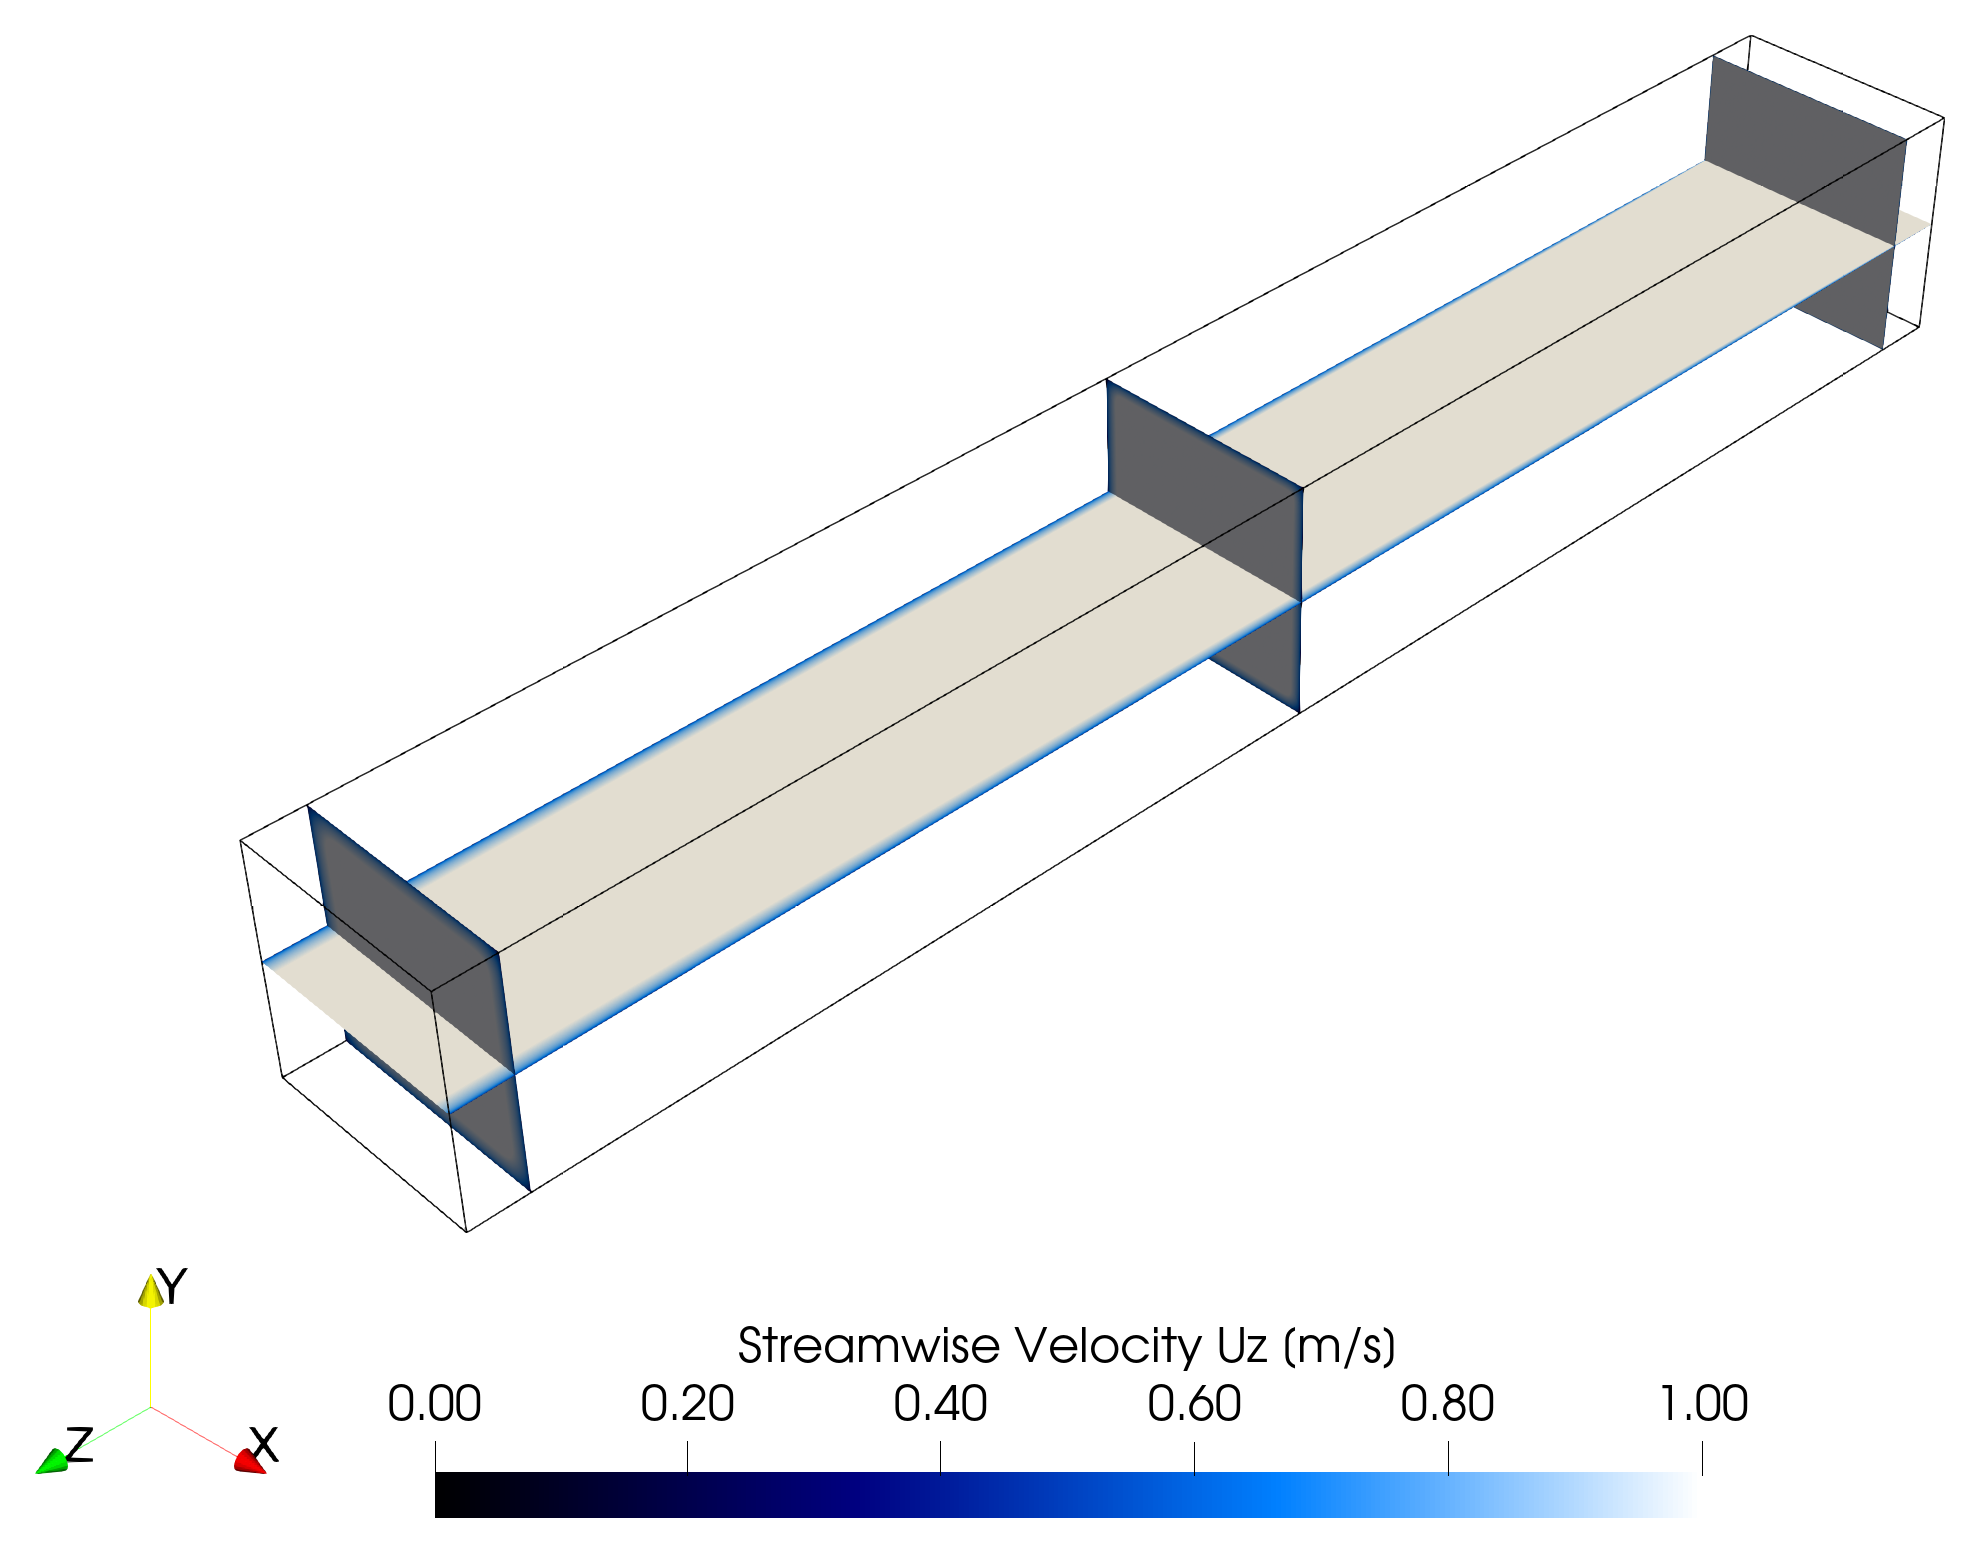
\includegraphics[width=\textwidth]{figures/fig7_boundary_layer_paraview_cropped.png}
        \captionof{figure}{Part I axial mid-plane $U_z$ and boundary layer growth ($z \in [0,1.50]\,\text{m}$).}
        \label{fig:p1_bl_contours}
    \end{minipage}\hfill
    \begin{minipage}[t]{0.47\textwidth}
        \centering
        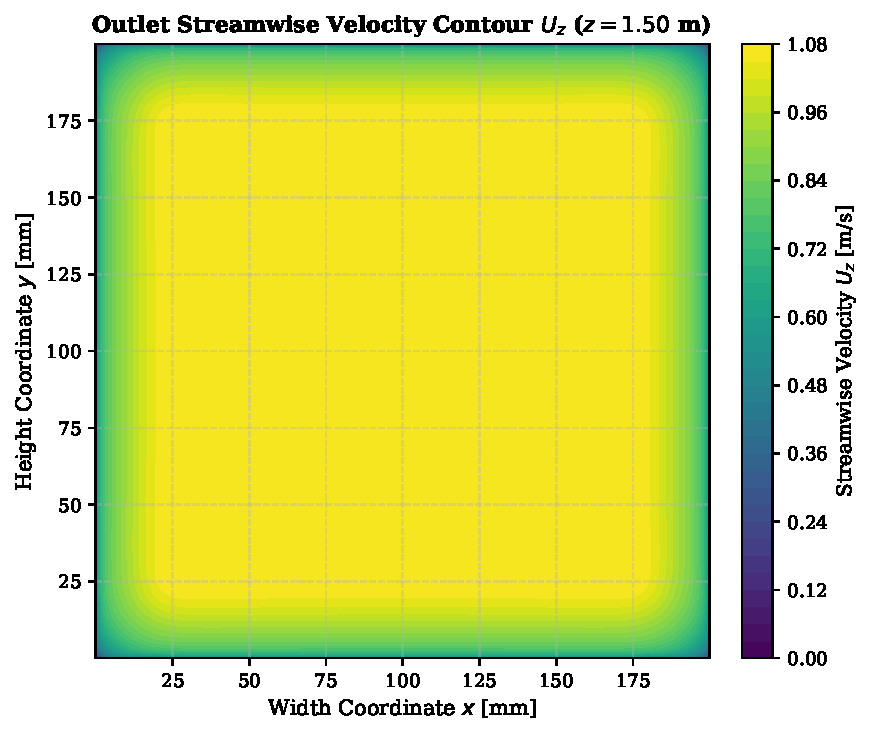
\includegraphics[width=\textwidth]{figures/fig5_cross_section_contour.pdf}
        \captionof{figure}{Part I cross-sectional $U_z$ development from $z = 0$ to $1.50\,\text{m}$.}
        \label{fig:p1_cross}
    \end{minipage}
\end{figure}

\begin{figure}[htbp]
    \centering
    \begin{minipage}[t]{0.49\textwidth}
        \centering
        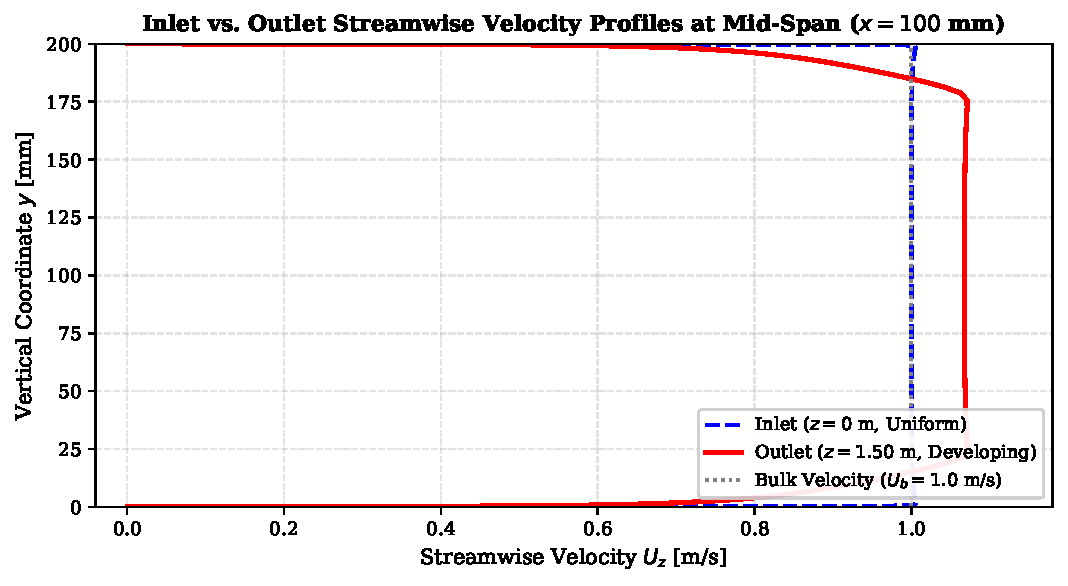
\includegraphics[width=\textwidth]{figures/fig1_velocity_profiles.pdf}
        \captionof{figure}{Part I wall-normal $U_z(y)$ profiles across axial stations.}
        \label{fig:p1_vel_press}
    \end{minipage}\hfill
    \begin{minipage}[t]{0.49\textwidth}
        \centering
        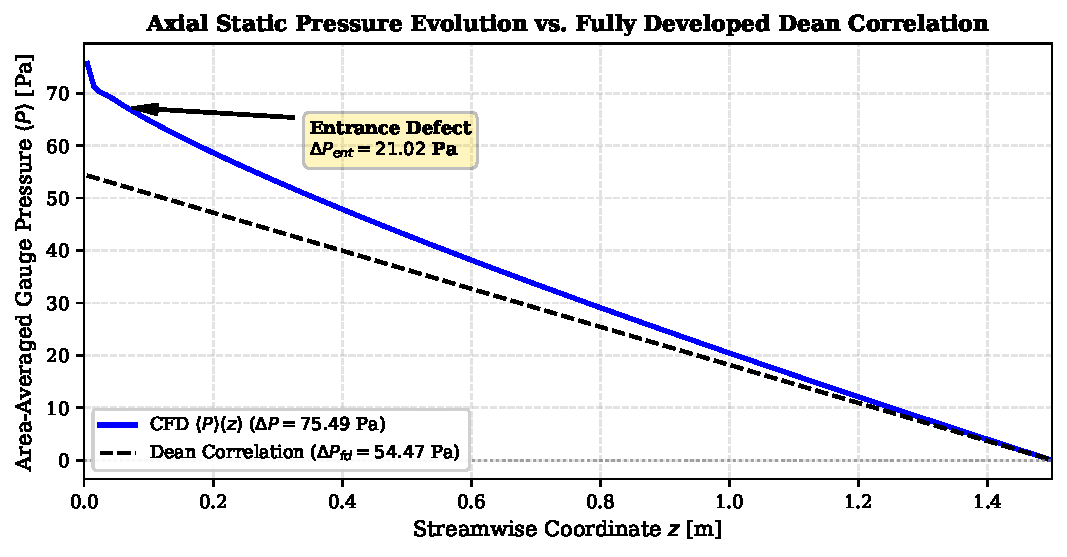
\includegraphics[width=\textwidth]{figures/fig3_axial_pressure_drop.pdf}
        \captionof{figure}{Part I area-averaged static gauge pressure $\langle P \rangle(z)$ vs.\ Dean.}
        \label{fig:p1_press}
    \end{minipage}
\end{figure}

\begin{figure}[htbp]
    \centering
    \begin{minipage}[t]{0.48\textwidth}
        \centering
        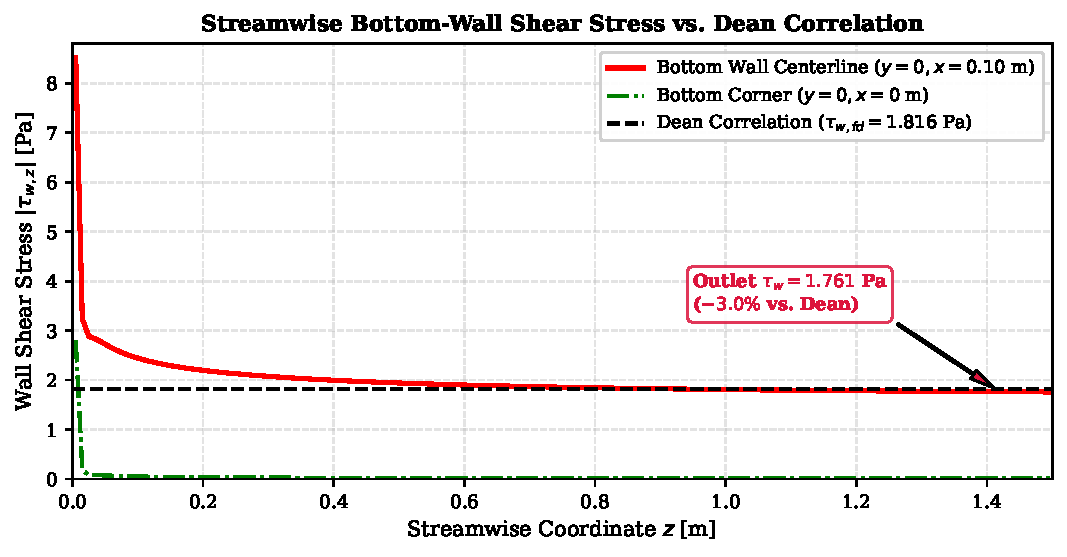
\includegraphics[width=\textwidth]{figures/fig4_wall_shear_stress.pdf}
        \captionof{figure}{Part I bottom-wall centerline $\tau_{w,z}(z)$ vs.\ Dean.}
        \label{fig:p1_shear}
    \end{minipage}\hfill
    \begin{minipage}[t]{0.50\textwidth}
        \centering
        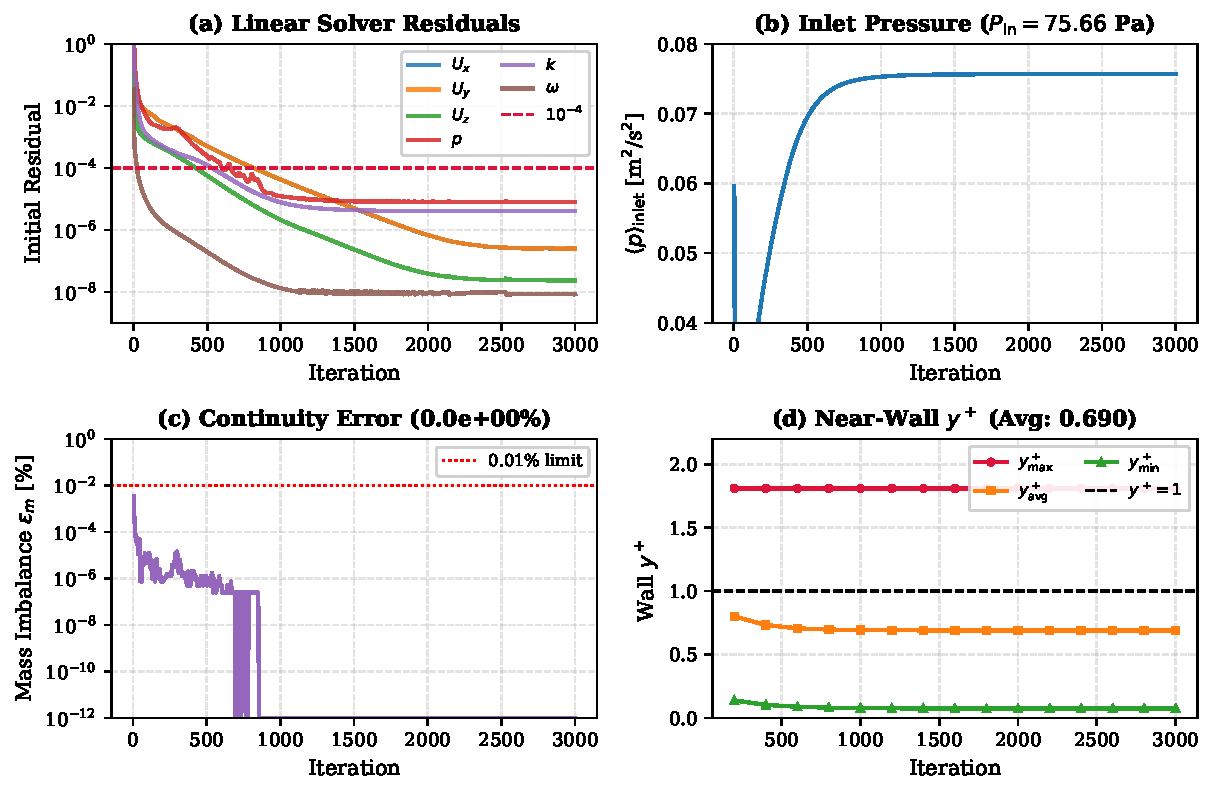
\includegraphics[width=\textwidth]{figures/fig6_convergence_and_verification.pdf}
        \captionof{figure}{Part I solver residual and mass/pressure convergence.}
        \label{fig:p1_conv}
    \end{minipage}
\end{figure}
\FloatBarrier

% =============================================================================
% SECTION 2: PART II
% =============================================================================
\section{Part II: Steady Flow Over a Surface-Mounted Cube (\texttt{simpleFoam})}

\textbf{Obstacle Setup, Mesh Sensitivity, and Steady Wake.} The $H_c = 0.05\,\text{m}$ obstacle ($x\in[0.075,0.125]\,\text{m}$, $y\in[0,0.050]\,\text{m}$, $z\in[0.400,0.450]\,\text{m}$; blockage $\beta = 6.25\%$, $Re_{H_c} = 55{,}991$) was carved out via \texttt{topoSet} and \texttt{subsetMesh} as a no-slip wall patch \texttt{cube}. Refining from Mesh A ($90\times 90\times 150$, $1{,}199{,}512$ fluid / $15{,}488$ removed cells, cube $y^+_{\text{avg/max}} = 12.45/41.99$, $\Delta P = 115.47\,\text{Pa}$, $|\mathbf{U}|_{\max} = 1.408\,\text{m/s}$) to Mesh B ($104\times 96\times 156$, $1{,}536{,}768$ fluid / $20{,}736$ removed cells, $25\,\mu\text{m}$ first cell at the cube) reduces $\Delta P$ by $3.2\%$ ($111.76\,\text{Pa}$) while resolving the cube boundary layer to $y^+_{\text{avg/max}} = \mathbf{0.929}/\mathbf{3.18}$ (duct walls $0.727/2.82$, non-ortho $0.00^\circ$, skew $4.34\times 10^{-11}$, $\varepsilon_m = \mathbf{2.50\times 10^{-6}\%}$). On Mesh B, the cube adds $\Delta P_{\text{cube}} = \mathbf{+36.27\,\text{Pa}}$ ($+48.05\%$, $K_{\text{cube}} = 0.0725$, $p_{\max}/p_{\min} = +607.18/{-}452.54\,\text{Pa}$), accelerates flow to $|\mathbf{U}|_{\max} = \mathbf{1.3304\,\text{m/s}}$, and produces an upstream horseshoe separation of $L_{\text{sep,up}} = \mathbf{52.98\,\text{mm}}$ ($1.06\,H_c$ at $z = 0.3470\,\text{m}$) plus a downstream recirculation bubble of $L_r = \mathbf{175.11\,\text{mm}}$ ($3.50\,H_c$, reattachment $z_R = 0.6251\,\text{m}$, $U_{z,\min} = -0.7135\,\text{m/s}$), with $k_{\max} = \mathbf{0.08458\,\text{m}^2/\text{s}^2}$ and peak cube wall shear $|\boldsymbol{\tau}_w|_{\max,\text{cube}} = \mathbf{50.64\,\text{Pa}}$ ($|\tau_x|_{\max} = 43.78\,\text{Pa}$) (Table~\ref{tab:p2_all}, Figures~\ref{fig:p2_pressure}--\ref{fig:p2_wake}).

\begin{table}[htbp]
    \centering
    \caption{Part II mesh sensitivity (Mesh A vs.\ Mesh B) and steady obstructed flow metrics on Mesh B.}
    \label{tab:p2_all}
    \small
    \resizebox{\textwidth}{!}{%
    \begin{tabular}{@{}l c c l c@{}}
        \toprule
        \textbf{Mesh Sensitivity Parameter} & \textbf{Mesh A} & \textbf{Mesh B (Final)} & \textbf{Steady Flow Metric (Mesh B)} & \textbf{Value} \\
        \midrule
        Grid / Fluid Cells & $1{,}199{,}512$ ($90\times 90\times 150$) & $\mathbf{1{,}536{,}768}$ ($104\times 96\times 156$) & Cube Loss $\Delta P_{\text{cube}}$ ($K_{\text{cube}}$) & $\mathbf{+36.27\,\text{Pa}}$ ($+48.05\%$, $K = 0.0725$) \\
        Removed Cube Cells & $15{,}488$ & $20{,}736$ & Pressure Extrema ($p_{\max}$ / $p_{\min}$) & $+607.18$ / $-452.54\,\text{Pa}$ \\
        Cube $y^+_{\text{avg}}$ / $y^+_{\max}$ & $12.45$ / $41.99$ & $\mathbf{0.929}$ / $\mathbf{3.18}$ & Max Speed $|\mathbf{U}|_{\max}$ / Backflow $U_{z,\min}$ & $\mathbf{1.3304}$ / $\mathbf{-0.7135\,\text{m/s}}$ \\
        Duct Wall $y^+_{\text{avg}}$ / $y^+_{\max}$ & --- & $0.727$ / $2.82$ & Upstream Sep.\ $L_{\text{sep,up}}$ ($z = 0.3470\,\text{m}$) & $\mathbf{52.98\,\text{mm}}$ ($\mathbf{1.06\,H_c}$) \\
        Total Duct $\Delta P$ & $115.47\,\text{Pa}$ & $\mathbf{111.76\,\text{Pa}}$ ($3.2\%\,\Delta$) & Wake Recirc.\ $L_r$ ($z_R = 0.6251\,\text{m}$) & $\mathbf{175.11\,\text{mm}}$ ($\mathbf{3.50\,H_c}$) \\
        Mass Imbalance ($\varepsilon_m$) & --- & $\mathbf{2.50\times 10^{-6}\%}$ & Peak TKE $k_{\max}$ / Cube $|\boldsymbol{\tau}_w|_{\max}$ & $\mathbf{0.08458\,\text{m}^2/\text{s}^2}$ / $\mathbf{50.64\,\text{Pa}}$ \\
        \bottomrule
    \end{tabular}}
\end{table}

\begin{figure}[htbp]
    \centering
    \begin{minipage}[t]{0.49\textwidth}
        \centering
        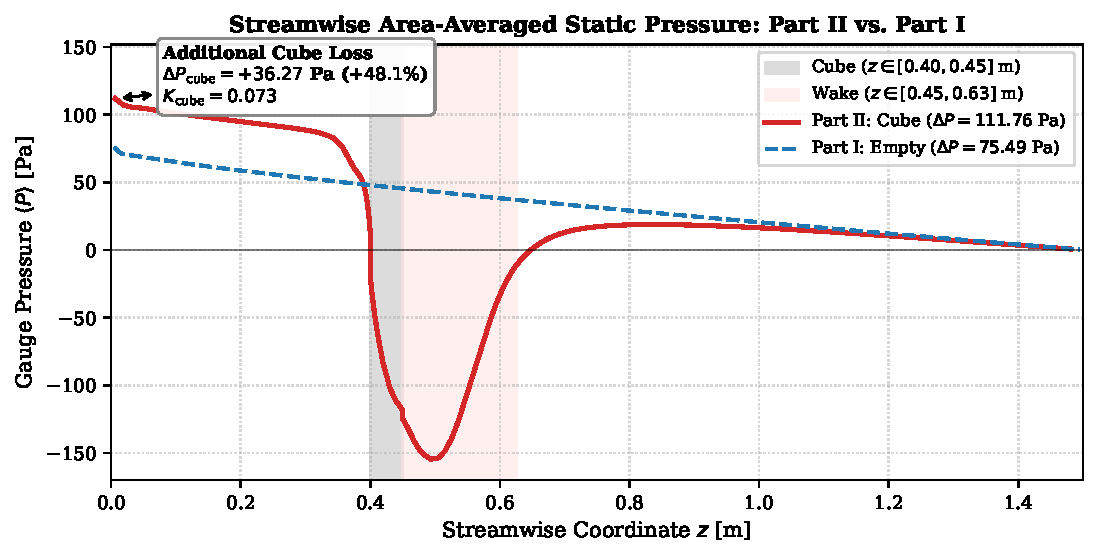
\includegraphics[width=\textwidth]{figures/fig_part2_pressure_drop.pdf}
        \captionof{figure}{Part II vs.\ Part I area-averaged static gauge pressure $\langle P \rangle(z)$.}
        \label{fig:p2_pressure}
    \end{minipage}\hfill
    \begin{minipage}[t]{0.49\textwidth}
        \centering
        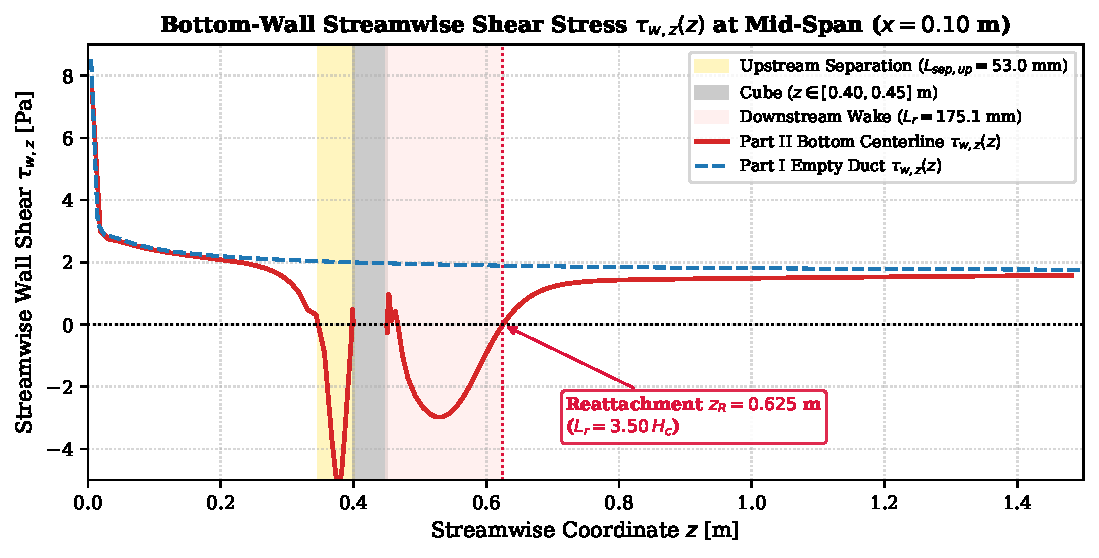
\includegraphics[width=\textwidth]{figures/fig_part2_wall_shear_and_wake.pdf}
        \captionof{figure}{Bottom-wall centerline $\tau_{w,z}(z)$ showing upstream separation and wake.}
        \label{fig:p2_shear}
    \end{minipage}
\end{figure}

\begin{figure}[htbp]
    \centering
    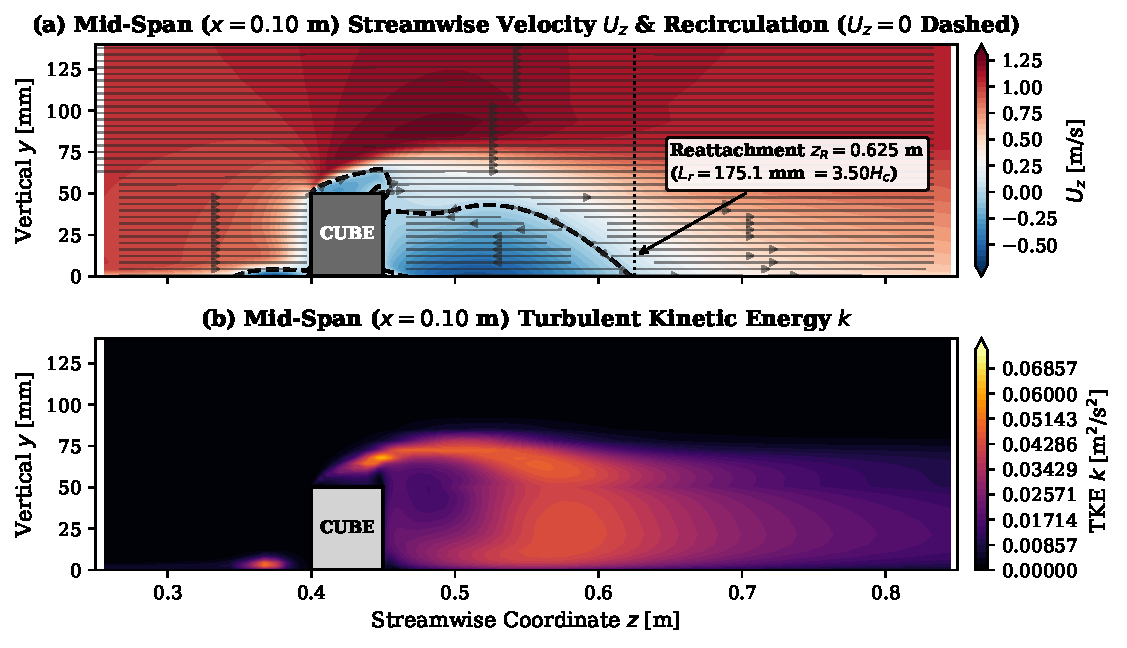
\includegraphics[width=0.90\textwidth]{figures/fig_part2_wake_and_separation.pdf}
    \caption{Part II mid-span ($x = 0.10\,\text{m}$) flow field: (a) $U_z$ streamlines and $U_z = 0$ contour; (b) Turbulent kinetic energy $k$.}
    \label{fig:p2_wake}
\end{figure}

\begin{figure}[htbp]
    \centering
    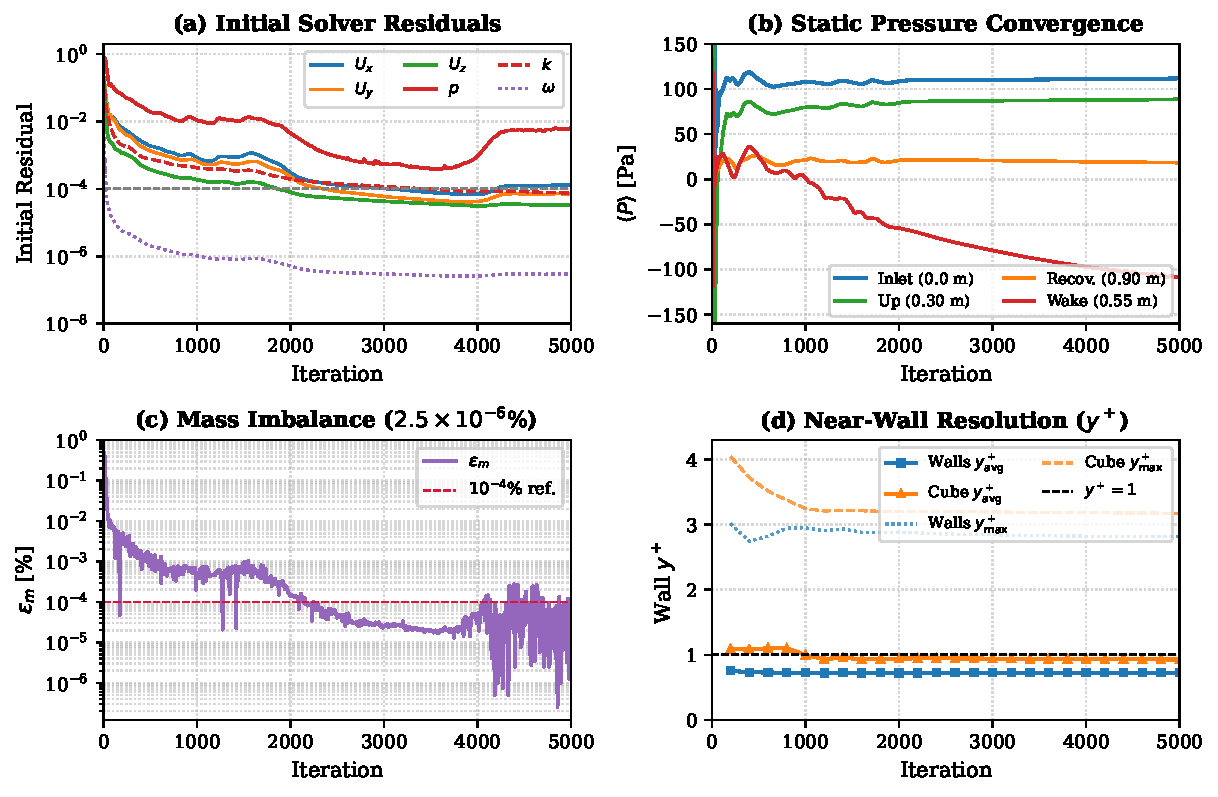
\includegraphics[width=0.72\textwidth]{figures/fig_part2_convergence.pdf}
    \caption{Part II steady solver convergence over $5{,}000$ SIMPLE iterations.}
    \label{fig:p2_conv}
\end{figure}
\FloatBarrier

% =============================================================================
% SECTION 3: PART III
% =============================================================================
\section{Part III: Transient Wake Development (\texttt{pimpleFoam})}

\textbf{Time-Step Adequacy, Vortex Shedding, and Steady vs.\ Time-Averaged Wake.} Initialized from steady Mesh B, \texttt{pimpleFoam} integrated $t \in [0, 2.00]\,\text{s}$ ($40.0\,H_c/U_b$) using blended Crank--Nicolson ($0.5$) and \texttt{adjustTimeStep} (\texttt{maxCo 6.0}), with statistics accumulated over $t \in [0.10, 2.00]\,\text{s}$. Adaptive $\Delta t$ settled at $\mathbf{7.72\times 10^{-5}\,\text{s}}$, keeping corner $\mathrm{Co}_{\max} = \mathbf{6.00}$ in the $25\,\mu\text{m}$ leading-edge cells while $\mathrm{Co}_{\text{mean}} = \mathbf{0.00928}$ ($0.030\text{--}0.045$ across the wake), $\varepsilon_m = \mathbf{2.93\times 10^{-5}\%}$, and $y^+_{\text{avg}} = 0.731$ (walls) / $0.945$ (cube). Across eight wake probes over $[0.50, 2.00]\,\text{s}$ (Table~\ref{tab:p3_probes}, Figure~\ref{fig:p3_probes}), FFT spectra identify primary lateral shedding at $f_x = \mathbf{2.000\,\text{Hz}}$ at \texttt{P5} ($\mathrm{St}_x = f_x H_c/U_b = \mathbf{0.1000}$; zero-crossing $1.886\,\text{Hz}$, $\mathrm{St}=0.0943$) and a streamwise harmonic at $f_z = \mathbf{2.667\,\text{Hz}}$ at \texttt{P4} ($\mathrm{St}_z = \mathbf{0.1333}$), consistent with wall-mounted cubes~\cite{martinuzzi1993}. Across $41$ saved snapshots, $L_r(t) \in \mathbf{167.53\text{--}193.11\,\text{mm}}$ ($\sigma = 5.60\,\text{mm}$), giving $\overline{L}_r = \mathbf{183.12\,\text{mm}}$ ($3.66\,H_c$, $\overline{z}_R = 0.6331\,\text{m}$), $\overline{L}_{\text{sep,up}} = \mathbf{45.26\,\text{mm}}$ ($0.91\,H_c$), peak resolved TKE $k_{\text{res},\max} = \mathbf{0.11114\,\text{m}^2/\text{s}^2}$ ($|\mathbf{u}'|_{\text{rms},\max} = \mathbf{0.4715\,\text{m/s}}$), $P'_{\text{rms},\max} = \mathbf{110.29\,\text{Pa}}$, and time-averaged $\overline{\Delta P} = \mathbf{135.57\,\text{Pa}}$ ($\overline{\Delta P}_{\text{cube}} = \mathbf{60.08\,\text{Pa}}$, $K_{\text{cube}} = 0.1202$, $+21.3\%$ total / $+65.6\%$ cube loss over Part II) (Table~\ref{tab:p1_p2_p3}, Figures~\ref{fig:p3_co}--\ref{fig:p3_comp}).

\begin{table}[htbp]
    \centering
    \caption{Part III probe locations, velocity/pressure statistics ($t \in [0.50, 2.00]\,\text{s}$), and Strouhal numbers.}
    \label{tab:p3_probes}
    \resizebox{\textwidth}{!}{%
    \begin{tabular}{@{}l c c c c c l@{}}
        \toprule
        \textbf{Probe \& Region} & \textbf{Coords $(x,y,z)$ [m]} & $\overline{U}_z \pm U_{z,\text{rms}}$ [m/s] & $U_x$ \textbf{Range [m/s]} & $\overline{P}$ \textbf{[Pa]} & $f_{\text{dom}}$ \textbf{[Hz]} & $\mathrm{St} = f H_c / U_b$ \\
        \midrule
        P0: Upstream Core & $(0.10, 0.025, 0.300)$ & $+0.9747 \pm 0.0002$ & $[-0.003, -0.002]$ & $+158.0$ & --- & Steady approach \\
        P1: Upstream Foot & $(0.10, 0.005, 0.380)$ & $+0.2444 \pm 0.0041$ & $[-0.097, -0.090]$ & $+407.9$ & --- & Quasi-steady foot \\
        P2: Above Cube Roof & $(0.10, 0.060, 0.425)$ & $+0.0176 \pm 0.0099$ & $[-0.030, +0.030]$ & $-284.8$ & $2.000$ & $\mathrm{St}_x = 0.1000$ \\
        P3: Near Wake & $(0.10, 0.025, 0.475)$ & $-0.2900 \pm 0.0376$ & $[-0.036, +0.003]$ & $-265.0$ & $1.333$ & $\mathrm{St}_x = 0.0667$ \\
        P4: Wake Core & $(0.10, 0.025, 0.550)$ & $-0.3972 \pm 0.0319$ & $[-0.057, +0.096]$ & $-228.5$ & $2.667$ & $\mathrm{St}_z = \mathbf{0.1333}$ \\
        P5: Reattachment & $(0.10, 0.025, 0.650)$ & $+0.2826 \pm 0.0577$ & $[-0.156, +0.280]$ & $+38.5$ & $2.000$ & $\mathrm{St}_x = \mathbf{0.1000}$ \\
        P6: Far Wake & $(0.10, 0.025, 0.850)$ & $+0.7318 \pm 0.0303$ & $[-0.093, +0.107]$ & $+26.0$ & $2.000$ & $\mathrm{St}_x = \mathbf{0.1000}$ \\
        P7: Lower Wall Wake & $(0.10, 0.003, 0.550)$ & $-0.5622 \pm 0.0259$ & $[-0.141, +0.054]$ & $-213.3$ & $2.000$ & $\mathrm{St}_x = \mathbf{0.1000}$ \\
        \bottomrule
    \end{tabular}}
\end{table}

\begin{table}[htbp]
    \centering
    \caption{Hydrodynamic comparison: Part I (empty), Part II (steady RANS), and Part III (time-averaged \& instantaneous URANS).}
    \label{tab:p1_p2_p3}
    \resizebox{\textwidth}{!}{%
    \begin{tabular}{@{}l c c c c@{}}
        \toprule
        \textbf{Metric} & \textbf{Part I (Empty)} & \textbf{Part II (Steady)} & \textbf{Part III (Time-Avg)} & \textbf{Part III (Inst.\ $2.0\,\text{s}$)} \\
        \midrule
        Total Duct Pressure Drop ($\Delta P$) & $75.49\,\text{Pa}$ & $111.76\,\text{Pa}$ & $\mathbf{135.57\,\text{Pa}}$ & $137.34\,\text{Pa}$ \\
        Additional Cube Loss ($\Delta P_{\text{cube}}$ / $K$) & --- & $36.27\,\text{Pa}$ / $0.0725$ & $\mathbf{60.08\,\text{Pa}}$ / $\mathbf{0.1202}$ & $61.85\,\text{Pa}$ / $0.1237$ \\
        Upstream Separation ($L_{\text{sep,up}}$) & --- & $52.98\,\text{mm}$ ($1.06\,H_c$) & $\mathbf{45.26\,\text{mm}}$ ($0.91\,H_c$) & $48.10\,\text{mm}$ ($0.96\,H_c$) \\
        Downstream Wake Length ($L_r$) & --- & $175.11\,\text{mm}$ ($3.50\,H_c$) & $\mathbf{183.12\,\text{mm}}$ ($3.66\,H_c$) & $180.74\,\text{mm}$ ($3.61\,H_c$) \\
        Max $|\mathbf{U}|_{\max}$ / Reverse $U_{z,\min}$ & $1.0673$ / $0.00\,\text{m/s}$ & $1.3304$ / $-0.7135\,\text{m/s}$ & $\mathbf{1.3152}$ / $\mathbf{-0.7500\,\text{m/s}}$ & $1.3233$ / $-0.7433\,\text{m/s}$ \\
        Modeled / Resolved $k_{\max}$ [$\text{m}^2/\text{s}^2$] & $0.0079$ / --- & $0.0846$ / $0.0000$ & $\mathbf{0.0825}$ / $\mathbf{0.1111}$ & $0.0828$ (modeled) \\
        Dominant Shedding ($\mathrm{St}_x$, $\mathrm{St}_z$) & --- & Steady & $\mathbf{0.1000,\; 0.1333}$ & $f_x = 2.00,\; f_z = 2.67\,\text{Hz}$ \\
        Mass Imbalance ($\varepsilon_m$) & $0.00\%$ & $2.50\times 10^{-6}\%$ & --- & $\mathbf{2.93\times 10^{-5}\%}$ \\
        \bottomrule
    \end{tabular}}
\end{table}

\begin{figure}[htbp]
    \centering
    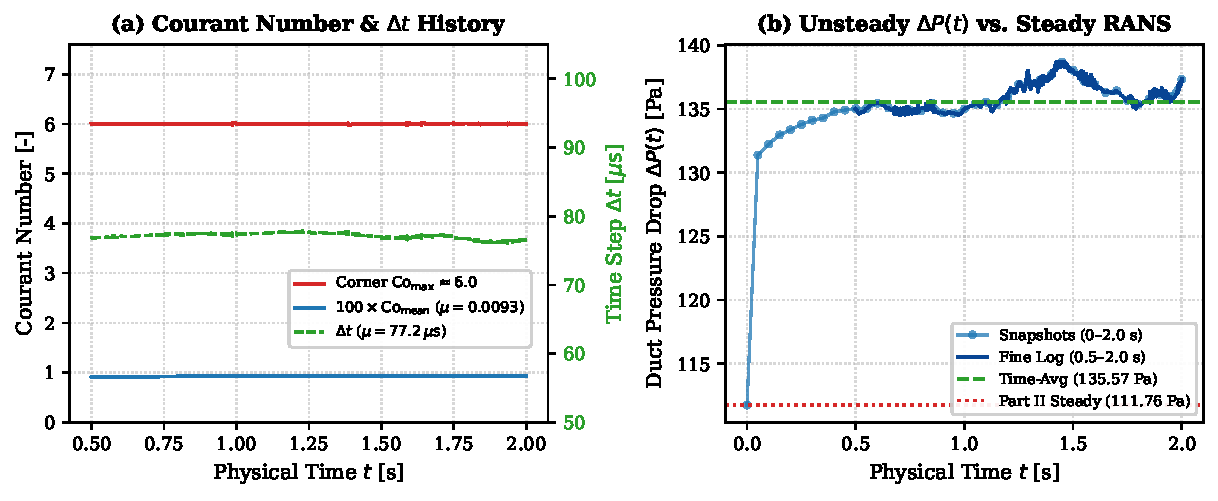
\includegraphics[width=0.94\textwidth]{figures/fig_part3_courant_and_convergence.pdf}
    \caption{Part III transient numerics: (a) $\mathrm{Co}_{\max}$, $\mathrm{Co}_{\text{mean}}$, and adaptive $\Delta t$ history; (b) Instantaneous $\Delta P(t)$ vs.\ Part II steady RANS.}
    \label{fig:p3_co}
\end{figure}

\begin{figure}[htbp]
    \centering
    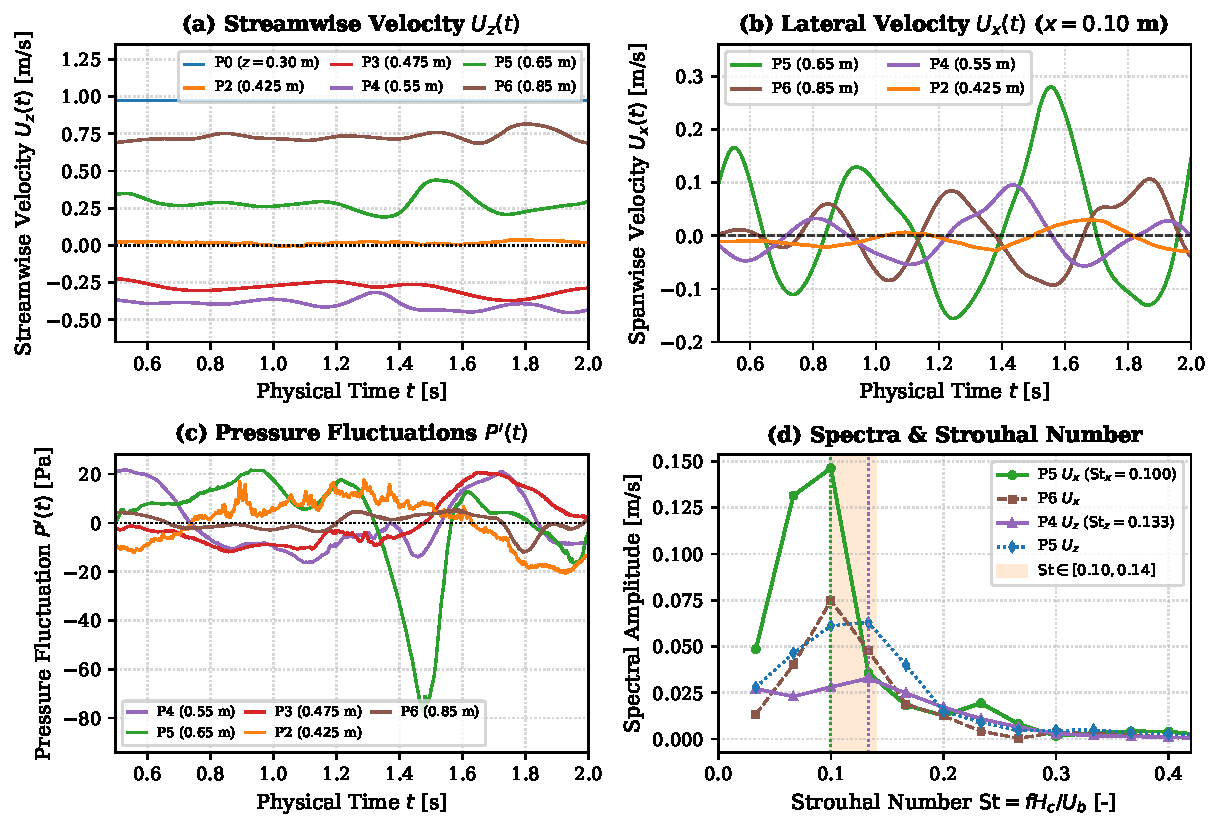
\includegraphics[width=0.80\textwidth]{figures/fig_part3_probe_histories_and_spectra.pdf}
    \caption{Part III probe records ($t \in [0.50, 2.00]\,\text{s}$): (a) $U_z(t)$; (b) $U_x(t)$; (c) $P'(t)$; (d) Spectra vs.\ Strouhal number.}
    \label{fig:p3_probes}
\end{figure}

\begin{figure}[htbp]
    \centering
    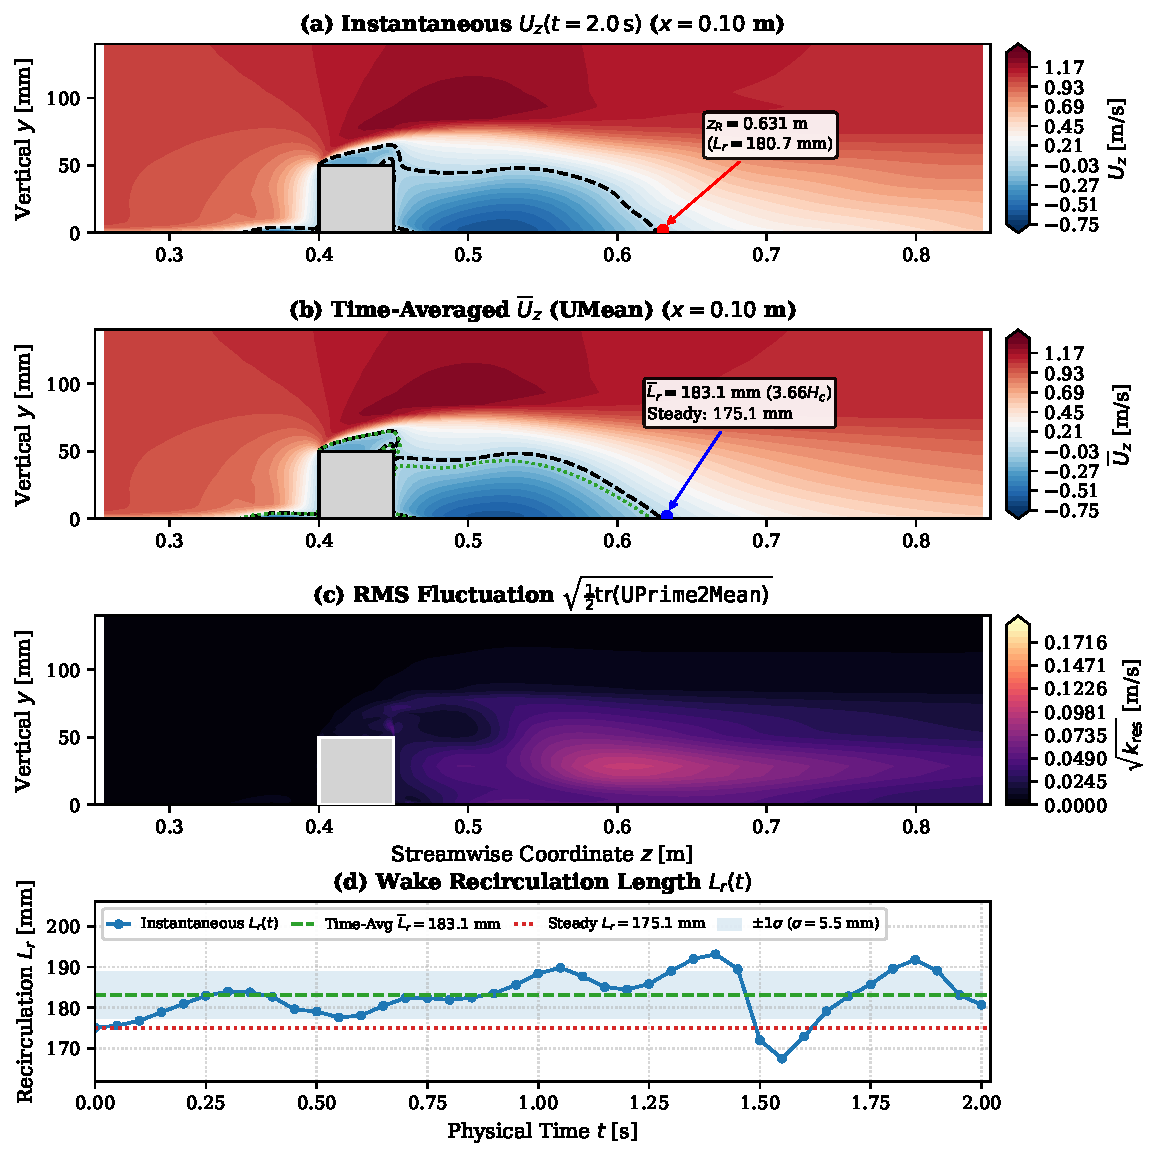
\includegraphics[width=0.78\textwidth]{figures/fig_part3_wake_evolution_and_recirculation.pdf}
    \caption{Part III wake evolution ($x = 0.10\,\text{m}$): (a) Instantaneous $U_z(2.0\,\text{s})$; (b) Time-averaged $\overline{U}_z$ vs.\ Part II (dotted); (c) RMS fluctuation $|\mathbf{u}'|_{\text{rms}}$; (d) $L_r(t)$ history.}
    \label{fig:p3_wake}
\end{figure}

\begin{figure}[htbp]
    \centering
    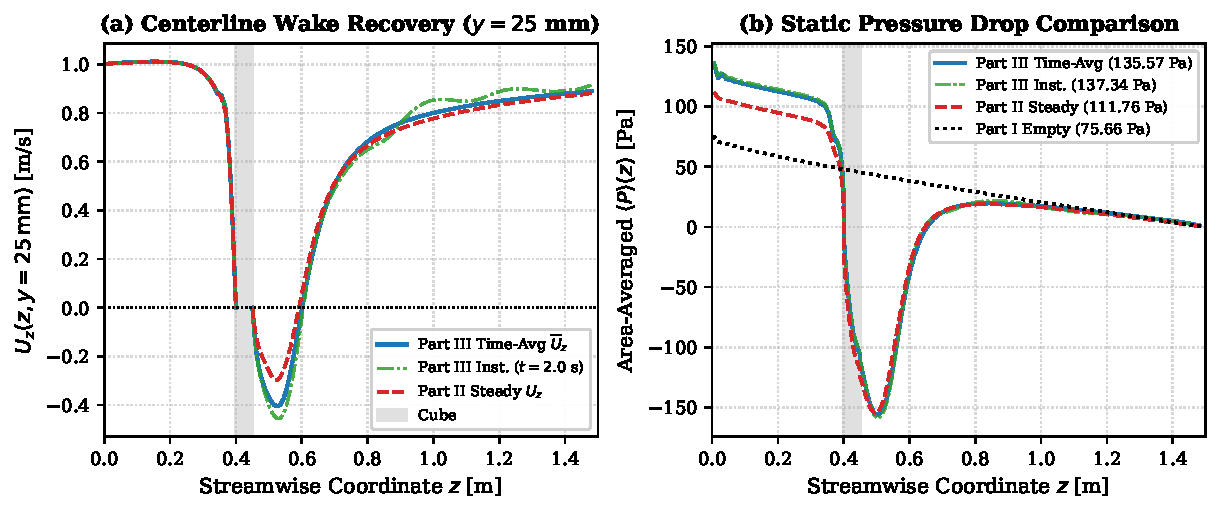
\includegraphics[width=0.92\textwidth]{figures/fig_part3_steady_vs_time_averaged_profiles.pdf}
    \caption{Part III time-averaged (\texttt{UMean}) vs.\ Part II steady comparison: (a) Wake centerline $U_z(z)$ ($y = 25\,\text{mm}$); (b) Area-averaged static pressure $\langle P \rangle(z)$.}
    \label{fig:p3_comp}
\end{figure}
\FloatBarrier

% =============================================================================
% SECTION 4: PART IV
% =============================================================================
\section{Part IV: Steady Conjugate Heat Transfer (\texttt{chtMultiRegionSimpleFoam})}

\textbf{Regions, Source Verification, and Energy Balance.} Using \texttt{splitMeshRegions}, Mesh B was partitioned into \texttt{fluid} ($1{,}536{,}768$ cells, $\rho=1000$, $c_p=4184$, $\mathrm{Pr}=6.135$, $T_{\text{in}}=298.15\,\text{K}$) and \texttt{solid} ($20{,}736$ cells, $V_s = 1.25\times 10^{-4}\,\text{m}^3$, $\rho_s=8000$, $c_{p,s}=500$, $\kappa_s=50\,\text{W/(m}\cdot\text{K)}$), with adiabatic outer duct walls and cube bottom. Volumetric heating $\dot{q} = 2.68\times 10^{10}\,\text{W/m}^3$ (\texttt{fvOptions}) supplies $Q_{\text{fvOptions}} = \mathbf{3.3500\,\text{MW}}$ ($\varepsilon_{\text{source}} = 0.084\%$ vs.\ analytical $Q_{\text{ref}} = 3.3472\,\text{MW}$ for $\Delta T = 20\,\text{K}$; exact rise $20.017\,\text{K}$). After $15{,}000$ iterations, $\varepsilon_m = \mathbf{1.48\times 10^{-5}\%}$, interface heat transfer is $Q_{\text{interface}} = \mathbf{3.3512\,\text{MW}}$ ($0.036\%$ source error; $\bar{q}'' = \mathbf{268.10\,\text{MW/m}^2}$ over $A_{\text{int}} = 0.0125\,\text{m}^2$), and coolant enthalpy removal is $Q_{\text{removed}} = \mathbf{3.3270\,\text{MW}}$ ($\varepsilon_Q = \mathbf{0.69\%}$), raising $T_{\text{in,mix}} \to T_{\text{out,mix}} = 298.15 \to \mathbf{318.03\,\text{K}}$ ($\Delta T_{\text{mix}} = \mathbf{19.88\,\text{K}}$). Solid temperatures reach $T_{\text{solid},\max} = \mathbf{178{,}171.6\,\text{K}}$, $T_{\text{solid,volAvg}} = \mathbf{113{,}705.6\,\text{K}}$, $T_{\text{solid},\min} = 13{,}771.3\,\text{K}$, while the interface averages $\bar{T}_{\text{int}} = \mathbf{68{,}489.5\,\text{K}}$ ($T_{\text{fluid},\max} = \mathbf{108{,}872.3\,\text{K}}$) and decays along the wake toward $298.15\,\text{K}$ freestream (Tables~\ref{tab:p4_balance}--\ref{tab:p4_faces}, Figures~\ref{fig:p4_conv}--\ref{fig:p4_wake}). Although bulk water carries away $3.35\,\text{MW}$ with only $\Delta T_{\text{mix}} = 19.88\,\text{K} < T_{\text{sat}}$, transferring $\bar{q}'' = 268.10\,\text{MW/m}^2$ across $0.0125\,\text{m}^2$ without phase change drives unphysically extreme surface temperatures ($T_{\text{fluid},\max} \gg 373.15\,\text{K}$), proving steady single-phase operation is impossible without boiling.

\begin{table}[htbp]
    \centering
    \caption{Part IV source verification, steady mass/energy balances, and global thermal metrics at iteration $15{,}000$.}
    \label{tab:p4_balance}
    \small
    \resizebox{\textwidth}{!}{%
    \begin{tabular}{@{}l c l c@{}}
        \toprule
        \textbf{Conservation / Verification Metric} & \textbf{Value} & \textbf{Temperature / Flow Metric} & \textbf{Value} \\
        \midrule
        Prescribed Power ($Q_{\text{fvOptions}} = \dot{q} V_s$) & $\mathbf{3.3500\,\text{MW}}$ & Solid Peak / Vol-Avg ($T_{\text{solid},\max}$ / $T_{\text{avg}}$) & $\mathbf{178{,}171.6}$ / $\mathbf{113{,}705.6\,\text{K}}$ \\
        Analytical Target ($Q_{\text{ref}}$, $\Delta T = 20\,\text{K}$) & $3.3472\,\text{MW}$ ($\varepsilon = 0.084\%$) & Solid Min Temp.\ ($T_{\text{solid},\min}$) & $13{,}771.3\,\text{K}$ \\
        Interface Heat Transfer ($Q_{\text{interface}}$) & $\mathbf{3.3512\,\text{MW}}$ ($\varepsilon = 0.036\%$) & Interface Area-Avg ($T_{\text{interface,avg}}$) & $\mathbf{68{,}489.5\,\text{K}}$ \\
        Coolant Heat Removal ($Q_{\text{removed}}$) & $\mathbf{3.3270\,\text{MW}}$ ($\varepsilon_Q = \mathbf{0.69\%}$) & Fluid Peak Temp.\ ($T_{\text{fluid},\max}$) & $\mathbf{108{,}872.3\,\text{K}}$ \\
        Mixed-Mean Temps ($T_{\text{in,mix}} \to T_{\text{out,mix}}$) & $298.15 \to \mathbf{318.03\,\text{K}}$ ($\Delta T_{\text{mix}} = \mathbf{19.88\,\text{K}}$) & Mean Interface Flux ($\bar{q}''$) & $\mathbf{268.10\,\text{MW/m}^2}$ \\
        Mass Imbalance ($\varepsilon_m$) & $\mathbf{1.48\times 10^{-5}\%}$ & Duct / Cube $y^+_{\text{avg}}$ ($y^+_{\max}$) & $0.730$ ($2.80$) / $0.918$ ($3.17$) \\
        \bottomrule
    \end{tabular}}
\end{table}

\begin{table}[htbp]
    \centering
    \caption{Part IV coupled interface breakdown across the five wetted cube faces ($A_i = 2.50\times 10^{-3}\,\text{m}^2$ each).}
    \label{tab:p4_faces}
    \small
    \resizebox{\textwidth}{!}{%
    \begin{tabular}{@{}l c c c c c c@{}}
        \toprule
        \textbf{Cube Face} & $Q_i$ \textbf{[MW]} & \textbf{Share [\%]} & $\bar{q}''_i$ \textbf{[MW/m$^2$]} & $\bar{T}_{\text{int},i}$ \textbf{[K]} & $T_{\text{int}}$ \textbf{Range [K]} & $h_{\text{eff},i}$ \textbf{[W/(m$^2\cdot$K)]} \\
        \midrule
        Front ($z = 0.40\,\text{m}$) & $0.8170$ & $24.38\%$ & $\mathbf{326.81}$ & $71{,}174$ & $[23{,}315,\; 100{,}131]$ & $4{,}610.7$ \\
        Top ($y = 0.05\,\text{m}$) & $0.5205$ & $15.53\%$ & $208.18$ & $65{,}023$ & $[13{,}794,\; 90{,}601]$ & $3{,}216.4$ \\
        Left ($x = 0.075\,\text{m}$) & $0.6375$ & $19.02\%$ & $255.00$ & $71{,}988$ & $[13{,}771,\; 107{,}531]$ & $3{,}557.0$ \\
        Right ($x = 0.125\,\text{m}$) & $0.6340$ & $18.92\%$ & $253.58$ & $72{,}808$ & $[14{,}274,\; 108{,}872]$ & $3{,}497.2$ \\
        Back ($z = 0.45\,\text{m}$) & $0.7423$ & $22.15\%$ & $296.91$ & $\mathbf{61{,}454}$ & $[13{,}776,\; 93{,}653]$ & $\mathbf{4{,}855.0}$ \\
        \midrule
        \textbf{Total / Mean} & $\mathbf{3.3512}$ & $\mathbf{100.00\%}$ & $\mathbf{268.10}$ & $\mathbf{68{,}489}$ & $[13{,}771,\; 108{,}872]$ & $\mathbf{3{,}931.5}$ \\
        \bottomrule
    \end{tabular}}
\end{table}

\begin{figure}[htbp]
    \centering
    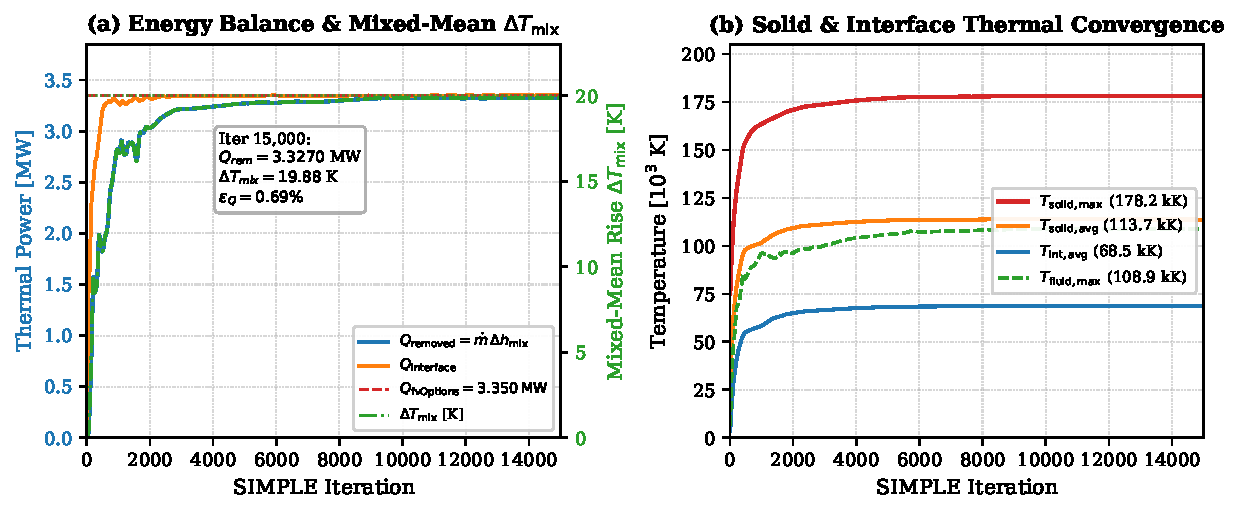
\includegraphics[width=0.94\textwidth]{figures/fig_part4_convergence_and_energy_balance.pdf}
    \caption{Part IV steady CHT convergence ($15{,}000$ iterations): (a) $Q_{\text{removed}}$, $Q_{\text{interface}}$, $Q_{\text{fvOptions}}$, and $\Delta T_{\text{mix}}$; (b) Solid, interface, and fluid temperature histories.}
    \label{fig:p4_conv}
\end{figure}

\begin{figure}[htbp]
    \centering
    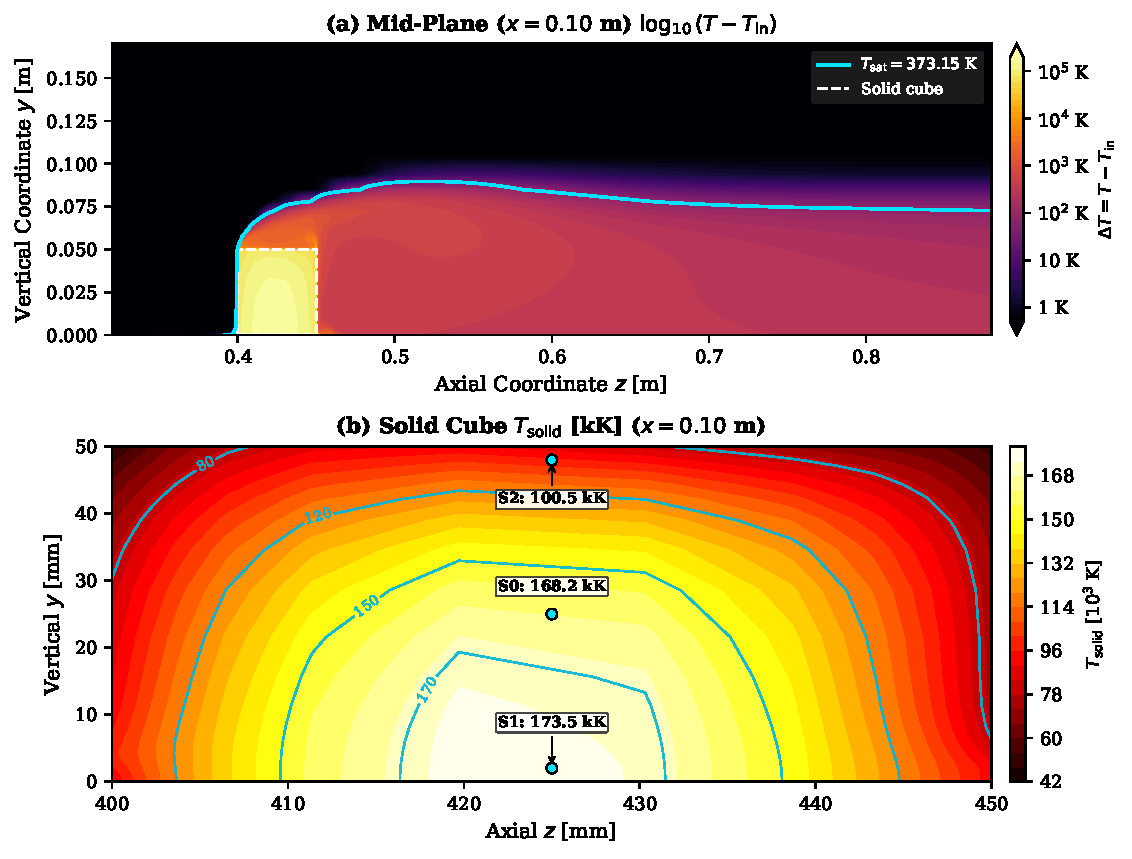
\includegraphics[width=0.84\textwidth]{figures/fig_part4_temperature_fields_and_solid.pdf}
    \caption{Part IV steady temperature fields ($x = 0.10\,\text{m}$): (a) $\log_{10}(T - T_{\text{in}})$ and boiling isotherm ($T_{\text{sat}} = 373.15\,\text{K}$); (b) Solid temperature $T_{\text{solid}}(z,y)$.}
    \label{fig:p4_fields}
\end{figure}

\begin{figure}[htbp]
    \centering
    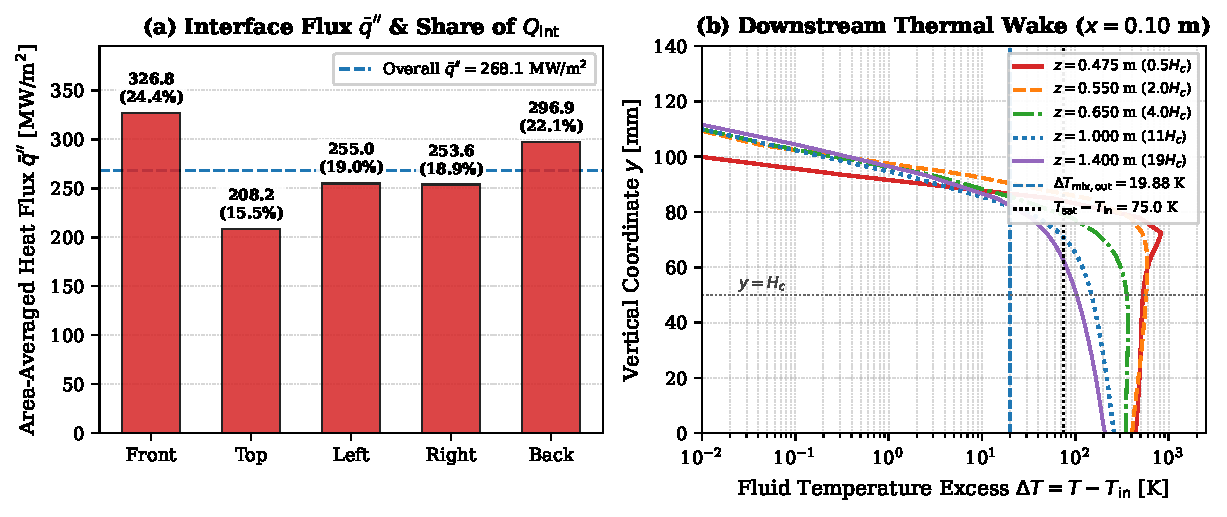
\includegraphics[width=0.94\textwidth]{figures/fig_part4_interface_flux_and_thermal_wake.pdf}
    \caption{Part IV coupled heat transfer: (a) Face-averaged $\bar{q}''$ and power share; (b) Downstream fluid thermal wake $\Delta T(y)$ profiles.}
    \label{fig:p4_wake}
\end{figure}
\FloatBarrier

% =============================================================================
% SECTION 5: PART V
% =============================================================================
\section{Part V: Transient Conjugate Heat Transfer (\texttt{chtMultiRegionFoam})}

\textbf{Setup, Boiling-Threshold Crossing ($t_{\text{boil}}$), and Transient Energy Balance.} \texttt{chtMultiRegionFoam} was integrated over $t \in [0, 20.00]\,\text{ms}$ ($400$ steps, $\Delta t = 50\,\mu\text{s}$, implicit Euler, PIMPLE 2/2) from uniform $T_0 = 298.15\,\text{K}$ and converged unheated flow, with continuous heating $\dot{q} = 2.68\times 10^{10}\,\text{W/m}^3$ ($Q_{\text{gen}} = 3.3500\,\text{MW}$) from $t = 0$. Numerical stability and conservation stay tight: $\varepsilon_m \le \mathbf{4.76\times 10^{-4}\%}$, $\mathrm{Co}_{\text{mean}} = \mathbf{0.00589}$ ($\mathrm{Co}_{\max} = 3.8533$), and solid diffusion $\mathrm{Di}_{\text{mean}} = \mathbf{0.07320}$ ($\mathrm{Di}_{\max} = 4.0006$). Relative to $p_{\text{out}} = 101.325\,\text{kPa}$ ($T_{\text{sat}} = 373.15\,\text{K}$; $p_{\text{in}} = 101.448\,\text{kPa}$), local peak interface pressure $p_{\text{if},\max} = \mathbf{101.945\,\text{kPa}}$ yields a Clausius--Clapeyron threshold $T_{\text{sat}}(p_{\text{if},\max}) = \mathbf{373.32\,\text{K}}$ ($100.17\,^\circ\text{C}$). Water first reaches $T_{\text{sat}}(p)$ at $\mathbf{t_{\text{boil}} = 12.39\,\text{ms}}$ ($0.012385\,\text{s}$; step $248$ at $12.40\,\text{ms}$ reaches $373.41\,\text{K}$; $1\,\text{atm}$ crossed at $12.36\,\text{ms}$; matches 1D analytical conduction benchmark $12.48\,\text{ms}$ within $\mathbf{0.79\%}$; first internal cell center at $12.5\,\mu\text{m}$ crosses at $16.51\,\text{ms}$) at the lower trailing corner of the left face, $(x, y, z) = (\mathbf{75.00}, \mathbf{0.81}, \mathbf{448.77})\,\text{mm}$. Over $20.00\,\text{ms}$ ($E_{\text{gen}} = 67.000\,\text{kJ}$), $\mathbf{99.63\%}$ of generated energy is stored in the solid ($E_{\text{solid}} = 66.7547\,\text{kJ}$), $\mathbf{0.34\%}$ in the fluid ($E_{\text{fluid}} = 226.26\,\text{J}$), and $Q_{\text{rem}} = 0.33\,\text{W}$ exits ($T_{\text{out,mix}} = 298.1500\,\text{K}$), achieving $\varepsilon_E = \mathbf{0.028\%}$ cumulative energy imbalance and $\varepsilon_P = \mathbf{0.054\%}$ instantaneous power imbalance ($\mathrm{d}E_{\text{solid}}/\mathrm{d}t = 3.3310\,\text{MW}$, $\mathrm{d}E_{\text{fluid}}/\mathrm{d}t = 17.15\,\text{kW}$, $Q_{\text{int}} = 18.97\,\text{kW}$) (Table~\ref{tab:p5_summary}, Figures~\ref{fig:p5_temps}--\ref{fig:p5_energy}).

\begin{table}[htbp]
    \centering
    \caption{Part V transient CHT metrics at boiling crossing ($12.40\,\text{ms}$) and run end ($20.00\,\text{ms}$).}
    \label{tab:p5_summary}
    \small
    \resizebox{\textwidth}{!}{%
    \begin{tabular}{@{}l c c l@{}}
        \toprule
        \textbf{Metric} & \textbf{At Crossing ($12.40\,\text{ms}$)} & \textbf{At Run End ($20.00\,\text{ms}$)} & \textbf{Basis / Assessment} \\
        \midrule
        Max Fluid Temp (Interface) & $373.41\,\text{K}$ ($100.26\,^\circ\text{C}$) & $419.51\,\text{K}$ ($146.36\,^\circ\text{C}$) & First crossing at $\mathbf{t_{\text{boil}} = 12.39\,\text{ms}}$ \\
        Max Fluid Temp ($12.5\,\mu\text{m}$ Cell Ctr) & $352.87\,\text{K}$ (interp.) & $392.42\,\text{K}$ ($119.27\,^\circ\text{C}$) & First cell-center crossing at $16.51\,\text{ms}$ \\
        Solid Cube $T_{\text{solid},\max}$ / $T_{\text{solid,volAvg}}$ & $381.23$ / $381.00\,\text{K}$ & $432.15$ / $431.66\,\text{K}$ & Near-adiabatic interior ramp ($6.70\,\text{K/ms}$) \\
        Interface $\bar{T}_{\text{int}}$ / Solid $T_{\text{solid},\min}$ & $372.88$ / $353.32\,\text{K}$ & $418.33$ / $383.15\,\text{K}$ & Corner cooling on wet faces \\
        Power Balance ($Q_{\text{gen}}$ / $\mathrm{d}E_{\text{solid}}/\mathrm{d}t$) & $3.3500$ / $3.3353\,\text{MW}$ & $3.3500$ / $3.3310\,\text{MW}$ & $99.43\%$ of $Q_{\text{gen}}$ stored in solid at $20\,\text{ms}$ \\
        Interface Flux $Q_{\text{int}}$ / Fluid Rate $\mathrm{d}E_f/\mathrm{d}t$ & $14.68$ / $15.26\,\text{kW}$ & $18.97$ / $17.15\,\text{kW}$ & $Q_{\text{rem}} = 0.33\,\text{W}$ ($\varepsilon_P = 0.054\%$ at $20\,\text{ms}$) \\
        Cumulative Energy ($E_{\text{gen}}$ / $E_{\text{solid}}$) & $41.54$ / $41.42\,\text{kJ}$ & $67.00$ / $66.75\,\text{kJ}$ & $99.63\%$ stored in solid cube \\
        Cumulative Fluid / Interface ($E_f$ / $\int Q_{\text{int}}\,\mathrm{d}t$) & $107.92$ / $116.35\,\text{J}$ & $226.26$ / $244.82\,\text{J}$ & $0.34\%$ in fluid ($\varepsilon_E = \mathbf{0.028\%}$) \\
        \bottomrule
    \end{tabular}}
\end{table}

\begin{figure}[htbp]
    \centering
    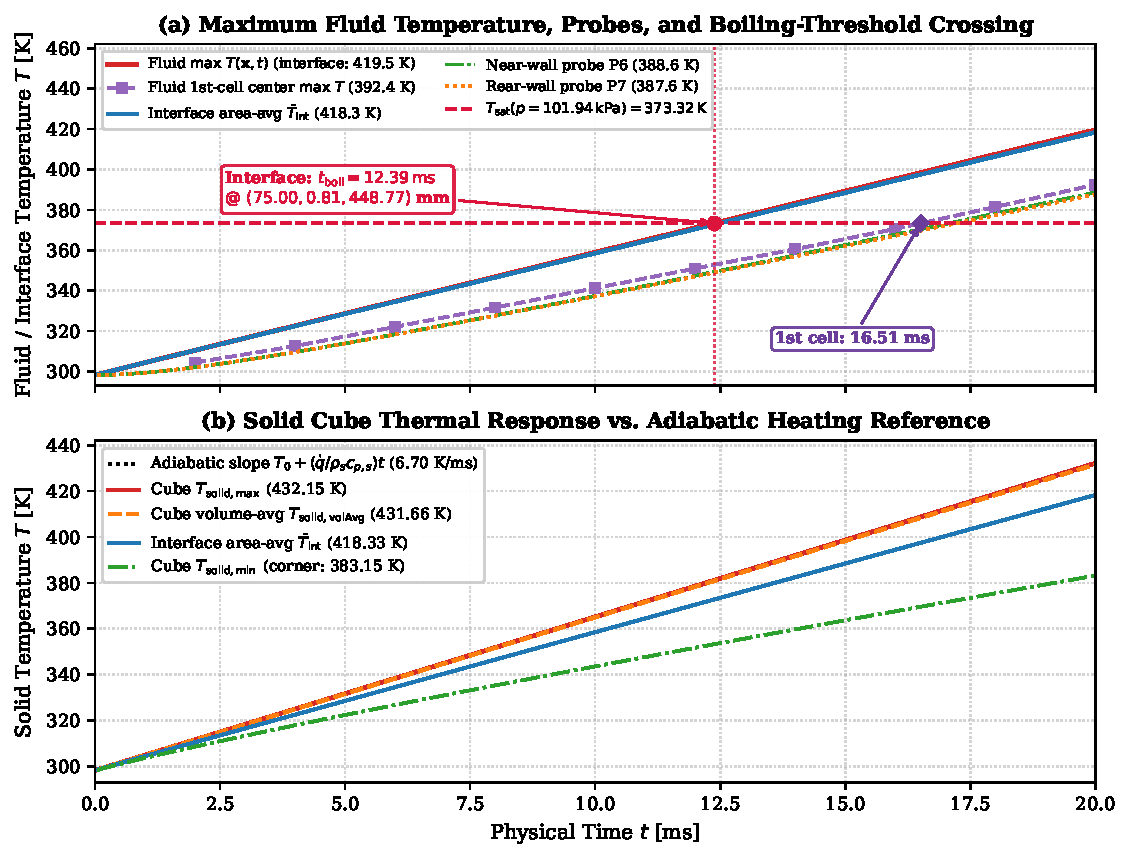
\includegraphics[width=0.84\textwidth]{figures/fig_part5_boiling_and_temperatures.pdf}
    \caption{Part V temperature histories ($t \in [0, 20.00]\,\text{ms}$): (a) Max interface, cell-center, $\bar{T}_{\text{int}}$, wake probes, and $t_{\text{boil}} = 12.39\,\text{ms}$; (b) Solid response vs.\ adiabatic ramp.}
    \label{fig:p5_temps}
\end{figure}

\begin{figure}[htbp]
    \centering
    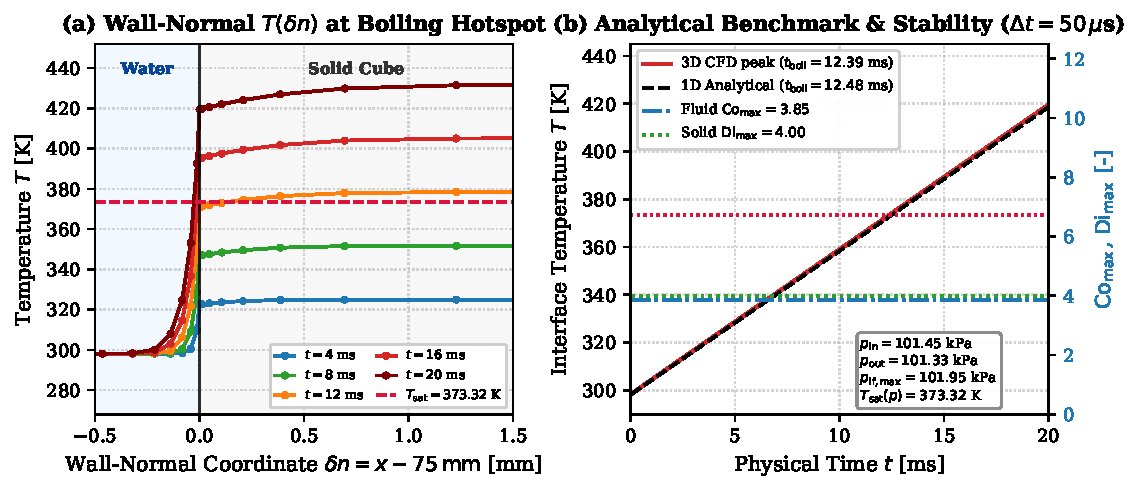
\includegraphics[width=0.86\textwidth]{figures/fig_part5_hotspot_and_numerics.pdf}
    \caption{Part V hotspot verification: (a) Wall-normal $T(\delta n)$ at $(75.00, 0.81, 448.77)\,\text{mm}$; (b) Interface peak vs.\ 1D analytical benchmark ($\mathrm{Co}_{\max} = 3.85$, $\mathrm{Di}_{\max} = 4.00$).}
    \label{fig:p5_hotspot}
\end{figure}

\begin{figure}[htbp]
    \centering
    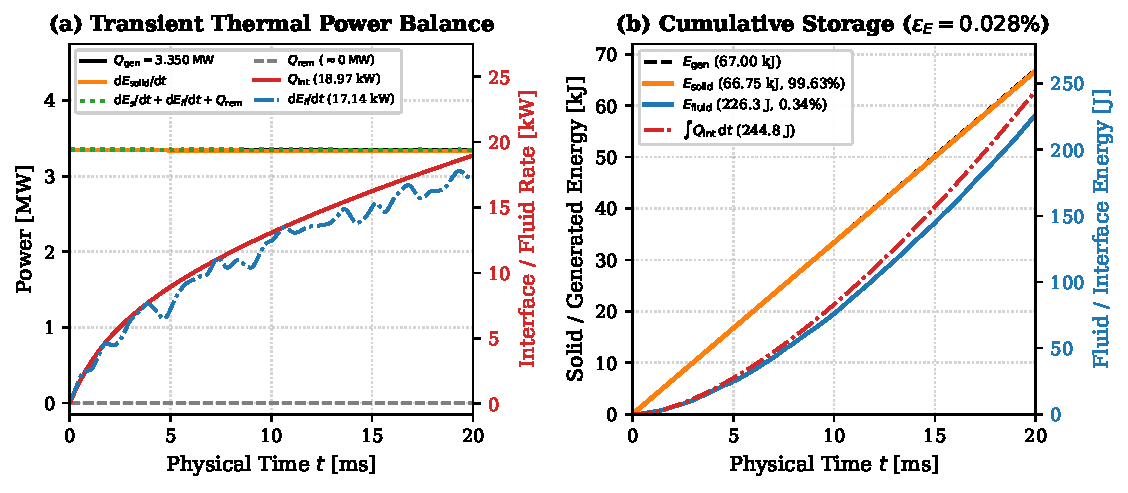
\includegraphics[width=0.86\textwidth]{figures/fig_part5_energy_balance_and_storage.pdf}
    \caption{Part V transient energy balance: (a) Instantaneous power balance; (b) Cumulative stored energy in solid ($99.63\%$) and water ($0.34\%$, $\varepsilon_E = 0.028\%$).}
    \label{fig:p5_energy}
\end{figure}

\textbf{Formal Conclusion.} Under single-phase non-boiling transient CHT initialized at $T_0 = 298.15\,\text{K}$ with continuous volumetric heating $\dot{q} = 2.68\times 10^{10}\,\text{W/m}^3$, local water saturation ($\max_{\text{fluid}} T \ge T_{\text{sat}}(p) = 373.32\,\text{K}$ at $p = 101.945\,\text{kPa}$) is first reached at $\mathbf{t_{\text{boil}} = 12.39\,\text{ms}}$ ($0.01239\,\text{s}$) at the lower trailing corner of the left cube face, $(75.00, 0.81, 448.77)\,\text{mm}$. Because boiling, latent heat, and vapor formation are not modeled in \texttt{chtMultiRegionFoam}, post-$t_{\text{boil}}$ temperatures ($419.51\,\text{K}$ at $20.00\,\text{ms}$) represent an idealized single-phase extrapolation past boiling onset.
\FloatBarrier

% =============================================================================
% SUMMARY & REFERENCES
% =============================================================================
\section*{Summary of Required Deliverables (Parts I--V)}
\begin{table}[htbp]
    \centering
    \footnotesize
    \begin{tabularx}{\textwidth}{@{}l l X@{}}
        \toprule
        \textbf{Part} & \textbf{Solver} & \textbf{Key Required Results} \\
        \midrule
        Part I & \texttt{simpleFoam} & $Re = 223{,}964$, $y^+_{\text{avg}} = 0.690$, $\varepsilon_m = 0.00\%$, $\Delta P = 75.49\,\text{Pa}$, $\tau_{w,\text{out}} = 1.761\,\text{Pa}$ ($-3.01\%$ vs.\ Dean) \\
        Part II & \texttt{simpleFoam} & $\varepsilon_m = 2.50\times 10^{-6}\%$, $\Delta P_{\text{cube}} = 36.27\,\text{Pa}$ ($+48.05\%$), $|\mathbf{U}|_{\max} = 1.3304\,\text{m/s}$, $L_{\text{sep,up}} = 52.98\,\text{mm}$, $L_r = 175.11\,\text{mm}$, $k_{\max} = 0.08458\,\text{m}^2/\text{s}^2$ \\
        Part III & \texttt{pimpleFoam} & $\Delta t = 7.72\times 10^{-5}\,\text{s}$, $\mathrm{Co}_{\text{mean}} = 0.00928$ ($\mathrm{Co}_{\max} = 6.00$), $\mathrm{St}_x = 0.1000$, $\mathrm{St}_z = 0.1333$, $\overline{L}_r = 183.12\,\text{mm}$, $\overline{\Delta P} = 135.57\,\text{Pa}$ \\
        Part IV & \texttt{chtMultiRegionSimpleFoam} & $\varepsilon_m = 1.48\times 10^{-5}\%$, $Q_{\text{fvOptions}} = 3.3500\,\text{MW}$, $Q_{\text{interface}} = 3.3512\,\text{MW}$, $\varepsilon_Q = 0.69\%$, $\Delta T_{\text{mix}} = 19.88\,\text{K}$, $\bar{q}'' = 268.10\,\text{MW/m}^2$, $T_{\text{solid},\max} = 178{,}171.6\,\text{K}$, $T_{\text{solid,avg}} = 113{,}705.6\,\text{K}$, $\bar{T}_{\text{int}} = 68{,}489.5\,\text{K}$ \\
        Part V & \texttt{chtMultiRegionFoam} & $\Delta t = 50\,\mu\text{s}$, $\mathrm{Co}_{\max} = 3.85$, $\mathrm{Di}_{\max} = 4.00$, $t_{\text{boil}} = 12.39\,\text{ms}$ at $(75.00, 0.81, 448.77)\,\text{mm}$ ($T_{\text{sat}} = 373.32\,\text{K}$ at $101.95\,\text{kPa}$), $E_{\text{solid}}(20\,\text{ms}) = 66.75\,\text{kJ}$ ($99.63\%$), $E_{\text{fluid}} = 226.26\,\text{J}$ ($0.34\%$), $\varepsilon_E = 0.028\%$ \\
        \bottomrule
    \end{tabularx}
\end{table}

\begin{thebibliography}{9}\small\setlength{\itemsep}{2pt}
\bibitem{dean1978} R.~B. Dean, ``Reynolds number dependence of skin friction and other bulk flow variables in two-dimensional rectangular duct flow,'' \emph{ASME J. Fluids Eng.}, 100(2), 215--223, 1978.
\bibitem{martinuzzi1993} R.~Martinuzzi and C.~Tropea, ``The flow around surface-mounted, prismatic obstacles placed in a fully developed channel flow,'' \emph{ASME J. Fluids Eng.}, 115(1), 85--92, 1993.
\bibitem{openfoam} OpenCFD Ltd., \emph{OpenFOAM User Guide}, 2024. \url{https://www.openfoam.com}
\end{thebibliography}

\end{document}
